\chapter{软横跨支柱容量校验}
\section{参数选取}
支柱容量是指支柱所能承受的、支柱不被破坏的最大弯矩,它取决于支柱本身的物理结构和材质特性,与支柱实际工作环境和工作状态无关。支柱容量与支柱的最大工作弯矩的比值称为支柱安全系数,一般取为2.0$\sim$3.0。

本设计横向承力索选用$GJ-70$镀锌钢绞线,上下部固定绳采用$GJ-50$镀锌钢绞线。其中,$GJ-70$型横向承力索的单位自重为$g_{ch}=6.15×10^{-3} kN/m$,直径为$d_{ch}=11mm$;$GJ-50$型上下部固定绳的单位自重为$g_{sc}=4.11×10^{-3}kN/m$,直径为$dsc=9mm$。

根据原始资料,车站正线悬挂采用JT-95+CT-120线索 ,车站站线悬挂采用JT-95+CT-110;接触网导高为6000mm;承力索补偿张力最大值为$T_{cmax}=15kN$,接触线补偿张力最大值为$T_{jmax}=10kN$;拉出值为$a=400mm$;第VIII分区的气象条件为:$t_{max}$=+40℃,$t_{min}$=-40℃,$t_b$=-5℃,$v_{max}$=30m/s,$v_b$=10m/s,b=10mm,γb=900kg/m3。
选择15、16 号软横跨支柱进行支柱容量计算,并完成校验。

\section{最大负载的选择}
根据的计算结果可知,站线和正线的最大合成负载均出现在覆冰时,站线最大合成负载为$q_{max1}=21.914×10^{-3} kN/m$,正线最大合成负载为$q_{max2}=24.296×10^{-3} kN/m$。

因此软横跨的最大负载出现在覆冰时,故以该状态下软横跨各类负载对支柱产生的弯矩作为最大工作弯矩。

\section{覆冰时软横跨的垂直负载}
该软横跨示意图如\ref{fig:软横跨示意图}所示。
% TODO: \usepackage{graphicx} required
\begin{figure}[H]
	\centering
	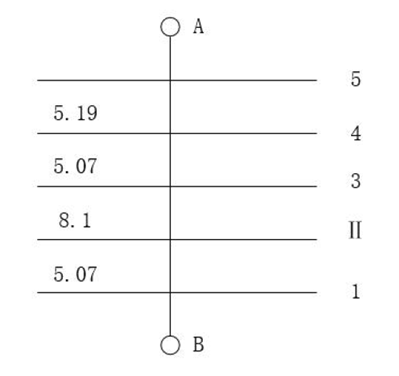
\includegraphics[width=0.7\linewidth]{figures/软横跨示意图}
	\caption{软横跨示意图}
	\label{fig:软横跨示意图}
\end{figure}
根据软横跨示意图,结合负载分析,得到软横跨垂直负载图如\ref{fig:软横跨垂直负债图}所示。
% TODO: \usepackage{graphicx} required
\begin{figure}[H]
	\centering
	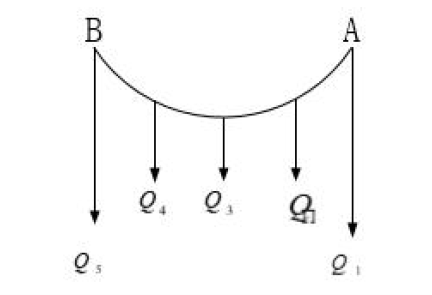
\includegraphics[width=0.7\linewidth]{figures/软横跨垂直负债图}
	\caption{软横跨垂直负债图}
	\label{fig:软横跨垂直负债图}
\end{figure}

选取软横跨左右跨距为l=60m,由A点至B点的软横跨节点分别为节点3、节点5、节点5、节点5、节点3。

\subsection{纵向悬挂作用于软横跨的垂直负载}
纵向悬挂施加到软横跨的垂直负载为:
\begin{align*}
	g_{q1}&=nq_{01}l+n(g_{cb}+g_{jb1})l
	\\
	&=2\times 13.91\times 10^{-3}\times 60+2\times (5.686+2.188)\times 10^{-3}\times 60
	\\
	&=2.614\mathrm{ kN}
	\\
	g_{q2}&=nq_{02}l+n(g_{cb}+g_{jb2})l
	\\
	&=2\times 16.088\times 10^{-3}\times 60+2\times (5.686+2.405)\times 10^{-3}\times 60
	\\
	&=2.901\mathrm{ kN}
	\\
	g_{q3}&=g_{q4}=\frac{1}{2}g_{q1}
	\\
	&=1.307\mathrm{ kN}
\end{align*}

\subsection{软横跨节点分布在各悬挂点的重量}
软横跨各节点重量为:
\[ J_1=J_2=650N,J_5=70N,J_8=610N \]
计算可得分布在各悬挂点的重量为:
\begin{align*}
	&J_{q1}=\frac{1}{2}J_2+J_5+\frac{1}{2}J_8=700\mathrm{ N}
	\\
	&J_{q2}=J_5+\frac{1}{2}J_8=375\mathrm{ N}
	\\
	&J_{q3}=J_5=70\mathrm{ N}
	\\
	&J_{q4}=\frac{1}{2}J_1+J_5=395\mathrm{ N}
\end{align*}
\subsection{软横跨自重分布在各悬挂点的重量}
软横跨自重分布在各悬挂点的重量计算式如下:
$$
p_{qi}=\frac{1}{2}(a_i+a_{i+1})(g_{ch}+2g_{sc})
$$
上式中,$a_i$表示与左侧相邻悬挂点的水平距离,$a_{i+1}$表示与左侧相邻悬挂点的水平距离。

从而可以计算得到软横跨自重分布在各悬挂点的重量分别为:
$$
p_{q1}=\frac{1}{2}(3.1+5.08)\times (6.15+2\times 4.11)\times 10^{-3}=58.77\times 10^{-3}\mathrm{ kN}
$$
$$
p_{q2}=\frac{1}{2}(7.5+5.08)\times (6.15+2\times 4.11)\times 10^{-3}=90.39\times 10^{-3}\mathrm{ kN}
$$
$$
p_{q3}=\frac{1}{2}(7.5+5.06)\times (6.15+2\times 4.11)\times 10^{-3}=90.39\times 10^{-3}\mathrm{ kN}
$$
$$
p_{q2}=\frac{1}{2}(3.1+5.06)\times (6.15+2\times 4.11)\times 10^{-3}=58.63\times 10^{-3}\mathrm{ kN}
$$

\subsection{各悬挂点的总负载}
根据以上计算结果可得各悬挂点的垂直总负载为:
\begin{align*}
	q_1&=g_{q1}+J_{q1}+p_{q1}
	\\
	&=2.614+0.7+0.05877
	\\
	&=3.373\mathrm{ kN}
	\\
	q_2&=g_{q2}+J_{q2}+p_{q2}
	\\
	&=2.901+0.375+0.09039
	\\
	&=3.366\mathrm{ kN}
	\\
	q_3&=g_{q3}+J_{q3}+p_{q3}
	\\
	&=1.307+0.07+0.09039
	\\
	&=1.467\mathrm{ kN}
	\\
	q_4&=g_{q4}+J_{q4}+p_{q4}
	\\
	&=1.307+0.395+0.05863
	\\
	&=1.761\mathrm{ kN}
\end{align*}
\section{覆冰时软横跨的水平负载}
\subsection{横向承力索张力}
根据覆冰时软横跨的垂直负载计算结果对悬挂点A列力矩平衡方程$\sum MA=0$,可得:
\begin{align*}
	F_B&=\frac{1}{L_1}\sum\nolimits_{i=1}^4{q_ix_i}
	\\
	&=\frac{3.373\times 20.74+3.366\times 15.66+1.467\times 8.16+1.761\times 3.1}{3.1+5.06+7.5+5.08+3.1}
	\\
	&=4.365\mathrm{ kN}
\end{align*}
根据垂直方向上的受力平衡$\sum F_y=0$得悬挂点A的垂直分离为:
\begin{align*}
	F_A&=\sum\nolimits_{i=1}^4{q_i-F_B}
	\\
	&=(3.373+3.366+1.467+1.761)-4.365
	\\
	&=5.602\mathrm{ kN}
\end{align*}
由试探法确定最低点,有:
$$
F_A-q_4-q_3>0
$$
$$
F_A-q_4-q_3-q_2<0
$$
因此认为荷载q2所在的悬挂点为最低点。

横向承力索弛度计算式为:
$$
f_{hmax}=H-H_s-C_{min}-0.1
$$
上式中,H为软横跨支柱高度,取为13m;$H_s$为上部固定绳至正线轨平面的高度,取为7.86m;$C_{min}$为吊弦最短长度,取为0.4m。

计算可得横向承力索的尺度为$f_{max}=4.64m$。

进而可得横向承力索张力大小为:
\begin{align*}
	T_h&=\frac{F_A\left( a_4+a_3+a_1 \right) -q_4\left( a_3+a_2 \right) -q_3a_2}{f_{max}}
	\\
	&=\frac{5.602\times (3.1+5.06+7.5)-1.761\times (5.06+7.5)-1.467\times 7.5}{4.64}
	\\
	&=11.769\mathrm{ kN}
\end{align*}
\subsection{上部固定绳的水平张力}
上部固定绳水平张力计算式为:
$$
T_s=4(P_{cb}l+T_{cz})
$$
上式中,$P_{cb}$为承力索覆冰时的单位风荷载,计算结果可得$P_{cb}=2.383×10^{-3} kN/m$;$T_{cz}$为承力索直线“之”字力,其计算式为:
\begin{align*}
	T_{cz}&=\frac{4T_{cmax}}{l}
	\\
	&=\frac{4\times 15}{60}\times 0.3
	\\
	&=0.3\mathrm{ k}N
\end{align*}
从而可得上部固定绳水平张力大小为$T_s=1.772 kN$。

\subsection{下部固定绳的水平张力}
下部固定绳水平张力计算式为:
$$
T_x=(3P_{jb120}+P_{jb110})l+4P_{jz}
$$
上式中,$P_{jb110}$为站线接触线覆冰时的单位风荷载,由计算结果可得$P_{jb110}=1.623×10^{-3} kN/m$;$P_{jb120}$为正线接触线覆冰时的单位风荷载,由计算结果可得$P_{jb120}=1.745×10^{-3} kN/m$;$T_{jz}$为接触线直线“之”字力,其计算式为:
\begin{align*}
	T_{jz}&=\frac{4T_{jmax}}{l}
	\\
	&=\frac{4\times 10}{60}\times 0.3
	\\
	&=0.2\mathrm{ kN}
\end{align*}
从而可得上下部固定绳水平张力大小为$T_x=1.197 kN$。
\subsection{支柱风负载}
支柱风负载的大小与覆冰风速以及支柱迎风面积有关,其计算式为:
$$
P_{zv}=0.625kFv_{b}^{2}\times 10^{-3}
$$
上式中,k取为1.25;F为支柱迎风面积,取为9.3 $m^2$;$v_b$为覆冰风速,根据原始资料可知$v_b=10 m/s$。

计算可得支柱风负载大小为$P_{zv}=0.723 kN$。

\section{软横跨支柱工作力矩计算与容量校验}
软横跨支柱最大工作力矩的计算式为:
$$
M_g=T_hH_h+T_sH_s+T_xH_x+\frac{1}{2}P_{zv}H_z
$$
上式中,$H_h$为横向承力索安装点至支柱基础平面的垂直距离,取为12.935m;$H_s$为上部固定绳至支柱基础平面的垂直距离,取为8.46m;$H_x$为下部固定绳至支柱基础平面的垂直距离,取为6.9m;$H_z$为软横跨支柱高度,取为13m。

代入上述计算结果,计算可得软横跨支柱最大工作力矩为$M_g=180.182 kN·m$。

计算容量为:
$$
M_R=1.5M_g=270.273\mathrm{ kN}\cdot m
$$
软横跨选用$H\frac{15}{300}$型钢筋混凝土支柱的容量为300 kN·m,大于计算容量,因此支柱容量满足要求。
